% Preamble
\documentclass[11pt]{article}

% Packages
%\usepackage{a4wide}
\usepackage[a4paper]{geometry}
\usepackage[english]{babel}
\usepackage[utf8]{inputenc}
\usepackage{xargs}                      % Use more than one optional parameter in a new commands
\usepackage[pdftex,dvipsnames]{xcolor}  % Coloured text etc.
\usepackage{graphicx} % Images etc.
\usepackage[hidelinks]{hyperref} % Makes citations clickable
\usepackage{amssymb}
\usepackage{amsmath}
\usepackage{mathtools} % e.g ":="

\usepackage[colorinlistoftodos,prependcaption,textsize=tiny]{todonotes}

\newcommandx{\unsure}[2][1=]{\todo[linecolor=orange,backgroundcolor=orange!25,bordercolor=orange,#1]{#2}}
\newcommandx{\Todo}[2][1=]{\todo[linecolor=yellow,backgroundcolor=yellow!25,bordercolor=yellow,#1]{#2}}

\renewcommand{\baselinestretch}{1.15} % line distance

\author{Nikolas Klug \\ Universität Augsburg}
\date{\today}
\title{To be determined}


\begin{document}
	\maketitle
	\newpage
	
	\begin{polyabstract}{Abstract}
	With well-performing 2D human pose estimators evolving over the last years, recent work focuses on inferring 3D poses from 2D poses.
	During the ECCV 2018 Workshops, Drover et al. presented such a 2D to 3D pose estimator in their work "Can 3D Pose be Learned from 2D Projections Alone?".
	Using a Generative Adversarial Network, their system is able to achieve state of the art results.
	On top of that, its main feature is that no 3D ground truth poses are required for training, which makes it especially attractive in applications where no ground truth data is available.
	
	In their proposed system, Drover et al. require the 2D input poses to be normalized in scale and position.
	The goal of this thesis is to analyze the effects of this normalization on the qualitative performance of the 3D pose estimation in that system.
	For this, baseline results for synthetically generated poses are established in a first step.
	Subsequently, the effects of normalization in position and scale are analyzed.
	Both the theoretical findings and the conducted experiments show that the normalization indeed negatively influences the measurable error.
	Since especially the normalization in position accounts for a significant increase in error, the system is modified to compensate for this.
	
	In addition to the analysis of the effects of normalization, an alternative loss function is proposed.
	It leverages high-level knowledge about the structure of human poses to produce improved results.
	With this new loss function, the error can be reduced by more than $7\%$. 
	
\end{polyabstract}

\pagebreak
\selectlanguage{german}
\begin{polyabstract}{Zusammenfassung}
	Da in den letzten Jahren leistungsstarke 2D Posenerkennungssysteme entwickelt wurden, liegt der Fokus der jüngsten Forschung darauf, aus diesen 2D Posen 3D Posen zu generieren.
	Während den ECCV 2018 Workshops haben Drover et al. in ihrer Arbeit \glqq Can 3D Pose be Learned from 2D Projections Alone?\grqq (in etwa \glqq Können 3D Posen ausschließlich von 2D Projektionen erlernt werden?\grqq) ein solches System vorgestellt, das für menschliche 2D Posen die dazugehörigen 3D Posen generiert.
	Mit Hilfe eines Generative Adversarial Networks gelingt es diesem System Ergebnisse zu erzielen, die dem aktuellen Stand der Technik entsprechen.
	Darüberhinaus bietet das System den großen Vorteil, dass für das Training keine 3D Grundwahrheitsposen benötigt werden.
	Dies macht das System besonders für Anwendungen attraktiv, in denen keine Grundwahrheitsdaten vorhanden sind.
	
	In dem von Drover et al. vorgestellten System müssen die 2D Eingabeposen in Größe und Position normalisiert sein.
	Das Ziel dieser Arbeit ist es, die Effekte dieser Normalisierung auf die qualitative Leistungsfähigkeit der 3D-Posengenerierung zu analysieren.
	Dafür werden als Erstes Ausgangsresultate für synthetisch generierte Posen ermittelt.
	Anschließend werden die Effekte der Größen- und Positionsnormalisierung analysiert.
	Sowohl die theoretische Untersuchung als auch die durchgeführten Experimente zeigen, dass die Normalisierung den messbaren Fehler negativ beeinflusst.
	Da insbesondere die Größennormalisierung für einen deutlichen Anstieg des Fehlers verantwortlich ist, wird das System so modifiziert, dass der zusätzliche Fehler kompensiert wird.
	
	Zusätzlich zur Analyse der Effekte der Posennormalisierung wird eine alternative Fehlerfunktion vorgestellt.
	Diese verwendet allgemeines Wissen über die Struktur menschlicher Posen, um verbesserte Ergebnisse zu erzielen.
	Mit der neuen Fehlerfunktion kann der Fehler um mehr als $7\%$ reduziert werden. 
\end{polyabstract}

\selectlanguage{english}
	\newpage
	
	\tableofcontents
	\newpage

	\section{Introduction}

Human pose estimation has gained a lot of attention in the last years.
With the emergence of models that are able to accurately estimate poses in real-time from RGB images only, pose tracking has now become more accessible than ever.
Systems like DeepCut \cite{pishchulin16}, the Stacked Hourglass architecture \cite{newell16} and most recently OpenPose \cite{cao18} are able to infer two dimensional (2D) human poses from RGB images with high precision.
With those well-performing 2D pose estimators, the next logical step is to estimate poses in three dimensions (3D).
For this, some end-to-end frameworks have been proposed, which estimate the 3D poses directly from RGB images \cite{pavlakos17, park16, mehta17, mehta17_2}.
Another approach is to split the task of 3D pose estimation into two subtasks \cite{drover18, martinez17, moreno-noguer16}:
2D pose estimation from RGB images and subsequent 3D pose estimation from the 2D poses.
This two-step pipeline benefits from the fact that the existing 2D pose estimators can be used for the first part, which means that 3D pose estimation is reduced to the second subtask, that is, the to 2D to 3D lifting.

Human pose estimation has been successfully applied in multiple areas.
In the medical field human pose estimation can help in detecting any movement related disorders.
\citet{aroeira16} use pose estimation to detect scoliosis in adolescents through the analysis of their postures.
In another work, \citet{khan18} use poses to monitor Vojta therapy, a form of therapy treating motor disabilities originating from neurological disorders.
Pose estimation is also necessary in future personal care robots that may be used in the context of assisted living \cite{richter15}.
Apart from applications in the medical field, an obvious application of human pose estimation is replacing the systems that are currently used for the task.
Concretely, those are Motion Capture (MoCap) systems used e.g. for animations and visualizations and RGBD cameras like Microsoft Kinect.
Not only are those systems expensive, but can also not be used in all environments (especially MoCap).
Here, pose estimation from RGB images only can provide a cheaper, more easily accessible alternative.
Human pose estimation can also be of help in the performance analysis of athletes in sports \cite{einfalt18, zecha19}.
Further applications include monitoring human behavior in surveillance scenarios, in working environments or elsewhere.

\subsection{"Can 3D Pose be Learned from 2D Projections Alone?"}

As explained above, recent work in the field of 3D pose estimation focuses on lifting 2D poses into three dimensions. 
In the paper "Can 3D Pose be Learned from 2D Projections Alone?", \citet{drover18} propose such a system.
On top of the state of the art results for the estimation, a major advantage of this system is that it can be trained in a weakly supervised manner.
It employs a Generative Adversarial Network \cite{goodfellow14} that relies only on 2D poses for training; no 3D ground truth data is required.
This makes the system particularly attractive, as compared to 2D ground truth data, acquiring 3D ground truth poses is notoriously harder (for a precise data collection, MoCap systems are usually required).

However, in this system, the 2D input poses are required to be normalized in scale and location before being lifted to 3D.
The objective of this thesis is an analysis of this system with respect to the influence of those normalization constraints on the error.
In addition to that, a modified loss function is proposed which enables an improved estimation of the 3D poses.

\subsection{Outline}

\autoref{sec:network} begins with a short introduction into Generative Adversarial Networks and perspective projection.
Those topics are the foundation of the pose estimation proposed by \citet{drover18}, which is presented and explained subsequently.

In \autoref{sec:data} the datasets used for evaluation -- which is mainly the Human3.6M dataset \cite{ionescu14} -- are presented.
As most pose estimation systems do not infer 3D poses in absolute scale, the estimated poses have to be transformed to be comparable to the ground truth poses.
The two main protocols that evolved in literature allow the application of different types of transformations to the estimated poses.
These protocols are analyzed and discussed.

Afterwards, in \autoref{sec:evaluation}, baseline errors for a rebuilt version of the system are established.
Those are required for the analysis of the effects of pose normalization, as well as for an evaluation of the modified loss function in later sections.
The system is evaluated for synthetically generated 2D poses and the monocular 2D poses included in the Human3.6M dataset.
In order to gain insights about the system's ability to generalize to unknown data, the system is also evaluated with poses from the TotalCapture dataset \cite{trumble17}.

In \autoref{sec:loss-function-modification}, a modified loss function for the generator is presented.
The new loss leverages high-level knowledge about human poses, which can be used by the generator to refine the estimated 3D poses.

\autoref{sec:effects-of-normalization} is the main part of this thesis.
Here, the two normalization constraints present in the 3D pose estimation system discussed in \autoref{sec:network} are analyzed.
The 2D input poses are expected to be normalized in location and scale.
By re-constructing the projections and re-projections of the poses during the estimation process, a theoretical lower bound for the minimal error is derived for both types of normalization.
Experiments are conducted in order to confirm the so-found lower bounds.

The results of the previous section show that especially the normalization in location introduces a significant additional error.
Hence, in \autoref{sec:network-adjusting} the system by \citet{drover18} is modified and trained such that the effects of normalization in location are diminished.

\autoref{sec:conclusion} concludes the thesis and provides a summary of the most important results.
	
	\section{Network architecture}
	\begin{itemize}
		\item basic principle of gans???
		\item Basic architecture used in the paper
		\item Mention batch norm not working?
		\item Projection and reprojection.
	\end{itemize}
	\section{Data}
	\begin{itemize}
		\item Dataset Human3.6m
		\item Original and augmented data
		\item Data used for training, evaluation and testing.
	\end{itemize}
	Assumptions:
	\begin{itemize}
		\item All 2d data can be scaled in a way that a norm limb is of length 0.1. 
		Problems with correct camera distance, see section \ref{sec:z-shift-error}
		\item All data was captured with the same camera distance.
	\end{itemize}
	\subsection{Evaluation Metrics}
	\subsubsection{Protocol 2}\label{sec:protocol2}
	%	
\section{Protocols}
\subsection{Protocol 1}
	\begin{itemize}
		\item Training: S1, S5, S6, S7, S8, S9 (commonly used, e.g. in \cite{chen17})
		\begin{itemize}
			\item \cite{drover18} do not use S9.
			\item The available code suggests that not every pose is used, but only such where at least one joint has moved by 40mm with respect to the former frame.
		\end{itemize} 			
		\item Evaluation: S11
		\begin{itemize}
			\item \cite{sun17} use every 64th frame (and also the code suggests this). If they only use the available code this would mean they use all four cameras.
			\item \cite{drover18} use ground truth 2d points for testing (might be the same as \cite{sun17})
			\item \cite{moreno-noguer16} use every 64th frame of the frontal view for testing
		\end{itemize}

		\item Error: \begin{itemize}
			\item \cite{drover18} use Mean per Joint Position Error (MPJPE) with scaling and rigid alignment to the ground truth skeleton (they don't mention which exactly)
			\item \cite{sun17} also use MPJPE after rigid alignment using Procrustes Analysis
			\item \cite{yasin16} use the MPJPE after alignment to the ground truth skeleton by a rigid transformation (they don't mention which exactly)
			\item \cite{kostrikov14} align the poses by a rigid transformation using \emph{least squares} before computing the MPJPE error
			\item \cite{tome17} perform a similarity transformation using a Procrustes Analysis
		\end{itemize}
		
	\end{itemize}
\subsection{Protocol 2}
	\begin{itemize}
		\item Training: S1, S5, S6, S7, S8
		\begin{itemize}
			\item Similar to protocol 1 the code suggests that not every pose is used, but only such where at least one joint has moved by 40mm with respect to the former frame.
			\item \cite{bogo16} evaluate on five different action sequences captured from the frontal camera
			\item \cite{tekin16, tekin17} use all camera views for training
		\end{itemize}
		\item Evaluation: S9, S11 
		\begin{itemize}
			\item \cite{sun17} use every 64th frame
			\item \cite{tekin16, tekin17} use all camera views for testing
			\item \cite{bogo16} evaluate on five different action sequences captured from the frontal camera
			\item \cite{moreno-noguer16} say they use all images for testing (whatever this means) 
		\end{itemize}
		\item Error: \begin{itemize}
			\item \cite{sun17} use MPJPE apparently without any alignment and scaling
			\item \cite{martinez17} align the root (central hip), they do not mention any scaling
			\item \cite{tome17} do not mention any alignment
			\item \cite{zhou18} scale the output such that the mean limb length is identical to the average value of all training subjects and align the root locations. Procrustes Analysis is not allowed.
			\item \cite{bogo16} apply a similarity transformation to align the reconstructed 3D joints via the Procrustes analysis on every frame
			\item \cite{zhou16} align the root locations and scale the output such that the mean limb length is identical to the average value of all training subjects. Procrustes alignment is not allowed.
			\item it seems that \cite{tekin16} also align the root nodes
			\item \cite{tekin17} use a Procrustes transformation before measuring the MPJPE
			\item \cite{pavlakos17} align the root joints
		\end{itemize}
	\end{itemize}

\subsection{Miscellaneous}
\begin{itemize}
	\item \cite{jahangiri17} evaluate using all subjects after a similarity transformation obtained by Procrustes alignment
\end{itemize}

\section{Questions and Problems}
\begin{itemize}
	\item It is sometimes not clear which 2d poses are used for testing.
	\item The transformations applied before calculating the error are not consistent within the protocols.
\end{itemize}


\section{Our approach}
	\subsection{Protocol 1}
		\begin{itemize}
			\item Training subjects: S1, S5, S6, S7, S8, S9
			\item Testing/Evaluation subjects: S11
			\item For now we train on all frames available, \emph{not} such where at least one joint has moved by 40mm
			\item For evaluation every 64th frame available for the according subjects is used
			\item Error metric: MPJPE
			\item Before calculating the error, the poses are transformed using a Procrustes Transformation and the root nodes are aligned
		\end{itemize}
	\subsection{Protocol 2}
		\begin{itemize}
			\item Training subjects: S1, S5, S6, S7, S8
			\item Testing/Evaluation subjects: S9, S11
			\item For now we train on all frames available, \emph{not} such where at least one joint has moved by 40mm
			\item For evaluation every 64th frame available for the according subjects is used
			\item Error metric: MPJPE
			\item Before calculating the error, the root nodes are aligned and the pose is scaled such that the mean limb length is identical to the average value of all training subjects
		\end{itemize}
 
	\subsection{Results for data}\label{sec:data-results}
	\begin{itemize}
		\item Results for self created data
		\item Results for original 2d data
	\end{itemize}
	\subsection{Different errors for different sets of joints}
		Using only 15 joints yields a much lower MPJPE than using 32 joints. Reasons: ...	
		From now on all numbers are calculated for 15 joint poses.
	\section{Part 1: MPJPE increase when shifting}
	
	Possible deviations of the assumptions about the three dimensional poses and how they are projected onto the image plane: Deviation in x and y direction, deviation in z direction, different focal length.
	
	We regard the system as a black box that takes a normalized set of two dimensional points as input and outputs the depths (the z coordinates) of the input points which then can be reprojected into three dimensional space.
	\subsection{Shifting along one image plane axis}
	\Todo{Add introduction to nomenclature and notation.}
	\label{sec:x-shift-error}
	\subsubsection{Theoretical analysis}
	\Todo{Properly define the pose and the camera.}
	Let $P_i=(x_i, y_i, z_i) \in \mathbb{R}^3$ and $f$ the focal length of a camera which is located at the origin along the x-y-plane and looks at $(0, 0, z)$, the location of the root joint. 
	Assume $P_i$ is shifted by $dx$ along the x axis.
	The x coordinate of the projected point on the image plane is
	\begin{equation}
		x_i^\mathrm{P} = f \frac{x_i + dx}{z_i} = f \frac{x_i}{z_i} + f \frac{dx}{z_i}\ .
	\end{equation}
	Subsequently all projected points are shifted along the x axis such that the root node which is located at $(0, 0, z)$ is in the origin of the image plane. That means:
	\begin{equation}
		\widetilde{x}_i^\mathrm{P} = f \frac{x_i}{z_i} + f \frac{dx}{z_i} - f \frac{dx}{z} 
		= f \frac{x_i}{z_i} + f dx (\frac{1}{z_i} - \frac{1}{z})
		= x_i^\mathrm{P} + f dx (\frac{1}{z_i} - \frac{1}{z})\ .
	\end{equation}
	After the system estimated the depth $\widetilde{z}_i$ of the point, it is reprojected into three dimensions. The resulting x coordinate is 
	\begin{equation}
		\widetilde{x}_i^\mathrm{R} = \frac{\widetilde{x}_i^\mathrm{P}}{f} \cdot \widetilde{z}_i
		= x_i \frac{\widetilde{z}_i}{z_i} + dx (\frac{1}{z_i} - \frac{1}{z}) \widetilde{z}_i
	\end{equation}
	The euclidean distance of the reprojected point to the original point is given by
	\begin{equation}
	\label{eq:delta-d}
		\Delta d_i = \left \| 
		\begin{pmatrix}
			\widetilde{x}_i^R - x_i \\
			\widetilde{z}_i - z_i
		\end{pmatrix}
		\right \|_2
	\end{equation}
	This expression takes on its minimum when 
	\begin{equation}
		\label{eq:minimum-distance}
		f(\widetilde{z}_i) = \left ( \widetilde{z}_i \cdot \left( \frac{x_i}{z_i} + dx \left( \frac{1}{z_i} - \frac{1}{z} \right) \right ) - x_i \right)^2 + ( \widetilde{z}_i - z_i ) ^2
	\end{equation}
	is minimal. 
	Substituting $a = \left( \frac{x_i}{z_i} + dx \left( \frac{1}{z_i} - \frac{1}{z} \right) \right )$ makes the equation more readable. 
	In order to obtain the optimal value for $\widetilde{z}_i$, \eqref{eq:minimum-distance} is differentiated by $\widetilde{z}_i$:
	\begin{equation}
		f'(\widetilde{z}_i) = 2 \cdot (\widetilde{z}_i a^2 - a x_i + \widetilde{z}_i - z_i)
	\end{equation}
	Setting this equal to zero gives
	\begin{align*}
		0 &= f'(\widetilde{z}_i) \\
		\Leftrightarrow \widetilde{z}_i & = \frac{a x_i + z_i}{1 + a^2} \ .
	\end{align*}
	Substituting this into \eqref{eq:delta-d} again yields a total minimal error of 
	\begin{equation}
		\label{eq:minimum-delta-d}
		\Delta d_i = \sqrt{\frac{(a z_i - x_i)^2}{a^2 + 1}}\
		= dx (1 -  \frac{z_i}{z}) \sqrt{\frac{1}{a^2 + 1}} .
	\end{equation}
	The MPJPE $\Delta d$ for a pose can then be calculated as the mean of all $\Delta d_i$s.
	
	\subsubsection{Experimental results}
		In practice, the observable error has the same approximate shape of this function, but is much smaller than the theoretical results.
		The reason for this is the scaling that is applied to the inferred poses during the evaluation of Protocol 2 (section \ref{sec:protocol2}).
		\unsure{Validate if this is really the case. Also see in what way it is proportional.}
		It appears that the average limb length of the inferred shifted poses is increasing monotonously with increasing offset $dx$.
		That means the poses are downsized by a factor $\alpha$ in all dimensions. 
		\Todo{Explain why} Therefore the actual error is $\Delta d' = \alpha \cdot \Delta d$.
		
		\begin{figure}[ht]
			\centering
			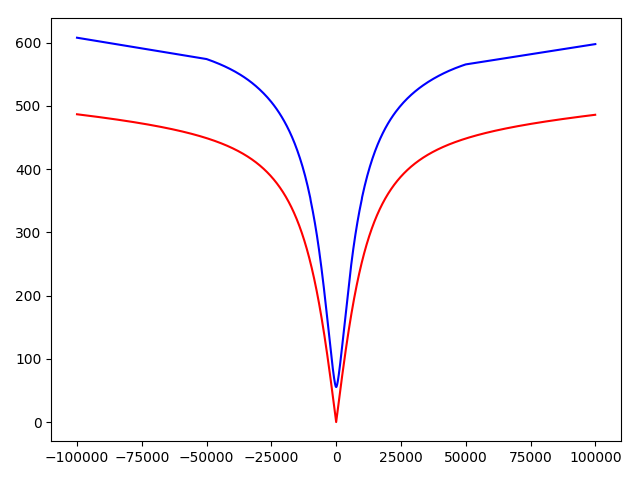
\includegraphics[scale=0.5]{images/x_shift_error.png}
			\caption{Plot of theoretical (red) and observed (blue) MPJPEs for different values of $dx$. 
				The theoretical errors are obtained by calculating the mean of the per pose errors $\alpha \Delta d$ for the evaluation data.}
			\Todo[inline]{Add axes titles, use proper image.
			Think about nice ways to display the values: Plot, Table?}
			\label{fig:x-shift-error}
		\end{figure}
	
		It is noticeable that the performance of the network is not worse than the theoretical results by a constant offset.
		For small deviations along the x axis the network seems to be able to compensate the error introduced by shifting.
		As $dx$ increases, so does the offset between the observed and the theoretical results until it seems to converge to a constant.
		This motivates adjusting not only how the inferred points are reprojected into three dimensions but also the input the network receives.
		This will be discussed further in section \ref{sec:network-adjusting}.
		
		As shown in section \ref{sec:data-results} the MPJPE for the original 2D poses is about \Todo{Check this number} 30mm higher than the one for the synthetically generated data.
		The simplest explanation for this is that the original 2D poses do not fulfill the constraints for the system.
		The camera is not centered on the root joint and also the camera distance is most certainly not exactly ten times the length of the norm limb.
		
		Numbers: ...
		
	\subsection{Shifting along the z axis}
	\label{sec:z-shift-error}
	\subsubsection{Theoretical analysis}
	Again consider a point $P_i=(x_i, y_i, z_i) \in \mathbb{R}^3$. Assume that $P_i$ is shifted by $dz$ along the z axis.
	The x coordinate of the projected point on the image plane is
	\begin{equation}
		x_i^\mathrm{P} = f \frac{x_i}{z_i + dz}
	\end{equation}
	The projected points are now scaled in a way that they have the same (arbitrary) scale.  Let $\alpha$ be the scale of the set of the original projected points and $\beta$ the one of the set of shifted projected points. The scaled projected point is given by
	
	\begin{equation}
			\widetilde{x}_i^\mathrm{P} = x_i^\mathrm{P} \cdot \frac{\alpha}{\beta} 
			= f \frac{x_i}{z_i + dz}\cdot \frac{\alpha}{\beta} 
	\end{equation}
	After the system estimates the depth $\widetilde{z}_i$ of each point, they are reprojected into 3 dimensional space.
	The reprojected points are given by
	\begin{equation}
		\widetilde{x}_i^\mathrm{R} = \frac{\widetilde{x}_i^\mathrm{P}}{f} \cdot \widetilde{z}_i
		= \frac{x_i}{z_i + dz}\cdot \frac{\alpha}{\beta}  \cdot \widetilde{z}_i
	\end{equation}
	Again we want to minimize equation \eqref{eq:delta-d}.
	If we define $a := \frac{x_i}{z_i + dz}\cdot \frac{\alpha}{\beta}$, the minimal value for $\Delta d$ is the same as in equation \eqref{eq:minimum-delta-d}.
	
	
	\subsubsection{Experimental results}
		This phenomenon is also affecting our ground truth data. The poses are all projected with a camera distance $ \text{length-of-norm-limb} \cdot 10$. 
		That means the length of the projected norm limb is not exactly $0.1$ but a bit smaller or bigger. 
		Like in the discussed above those projected poses are then normalized. 
		The system estimates the depths of the normalized pose and re-projects it assuming a perfect perspective projection. 
		It therefore does not consider the effect of small deviations in z direction.
		A way to fix this would be to calculate the perfect camera distance for each pose individually before projecting them onto the image plane.
		This is not very realistic though since one might be able to determine the camera's distance to a human approximately, but definitely not exactly. This phenomenon therefore is kind of inevitable.
		 
		
	\subsection{Total minimal error}
	
	Combining results of the previous two chapters
	
	\subsection{Alternation of the focal length}
	No difference
	
	
	\section{Part 2: Adjusting the network to tolerate shifting}
	\label{sec:network-adjusting}
	Error on original poses when training on "shift generator": 73.75
	\subsubsection{Original network with correct reprojection}
	
	\subsubsection{"New" network}
	Network that takes a shifted input.
	
	\section{Conclusion}
	This is the conclusion of the thesis.
	\newpage
	\bibliography{bibliography}
	\bibliographystyle{apalike}
	
\end{document}